%!TEX root = ../main.tex

\chapter{Partial contributions to clustering}\label{chap:contributions}
In this chapter, we present some work carried out during this thesis which have unfortunately not been able to be the subject of an in-depth study that can be published. The first part deals with the sparsity hypothesis of the precision matrices within a high dimensional Gaussian mixture and adapts the single-component Graphical Lasso from \citep{glasso07} to the mixture setting. In the second part, we assume that the weight vector of the mixture is sparse in order to obtain an estimator of the number of components in the mixture that is generally unknown. 

\section{Graphical Lasso for Gaussian mixtures}\label{chapgraphlasso}
As we saw in the previous sections, the number of free parameters in a full GMM with $K$ components in dimension $p$ are $(K-1)+Kp+Kp(p+1)/2$ which means, for instance, that for $K=5$ and $p=100$ we have $125704$ parameters to estimate. In this high dimensional setting, the EM algorithm experiences severe performance degradation. In particular, the inversion of the covariance matrices are one source of error. One way to circumvent these problems is to use regularization. To this end, we will make a structural assumption on the inverse of the covariance matrices, called precision or concentration matrices, of a component. The work presented in this chapter is inspired by \citep{glasso07}, \citep{banerjee}, \citep{yuanLin_graph} and \citep{meinshausen2006} where it is suggested to penalize the off-diagonal entries of the precision matrix of a Gaussian graphical model. We do an attempt to generalize this work to the Gaussian mixture model.

We consider $\bX=(X^{(1)},\dots,X^{(p)})$, a random vector admitting a $p$-dimensional normal distribution $\mathcal N(\bmu, \bSigma)$ with a non-singular $\bSigma$. One can construct an undirected graph $G=(V,E)$ with $p$ vertices corresponding to each coordinate and, $E=(e_{i,j})_{1\leq i < j \leq p}$, the edges between the vertices describing the conditional independence relation among $X^{(1)},\dots,X^{(p)}$. If in this graph, $e_{i,j}$ is absent in $E$ if and only if $X^{(i)}$ and $X^{(j)}$ are independent conditionally to the other variables $\{X^{(l)}\}$ with $l\neq i,j$ (denoted $X^{(i)} \ci X^{(j)}|X^{(l)}\, l\neq i,j$). Then $G$ is called the Gaussian concentration graph model for the Gaussian random vector $\bX$. 
This representation is particularly interesting in the study of the inverse of the covariance matrix. Let us denote $\bSigma^{-1}=\bOmega=(\omega_{i,j})$ the precision matrix. The entries of this matrix satisfy $\omega_{i,j}=0$ if and only if $X^{(i)} \ci X^{(j)}$ conditionally to all the other variables. We recall in the following lemma this well-known result

\begin{lemma}[Conditional independence in Gaussian concentration graph model]
Consider $\bX=(X^{(1)},\dots,X^{(p)})$, a p-dimensional random vector with a multivariate normal distribution $\mathcal N(\bmu, \bSigma)$, and set $\bSigma^{-1}=\bOmega=(\omega_{i,j})$. Then $X^{(i)} \ci X^{(j)}|\{X^{(l)}: l\notin\{i,j\}\} \iff \omega_{i,j}=0$ with $l\neq i,j$ 
\end{lemma}
\begin{proof}
This result can be found in \citep{edwards2000introduction}. Consider the density of $\bX$
\begin{equation}
  \varphi_{\bmu,\bSigma}(\bx)=\frac{1}{(2\pi)^{p/2}|\bSigma|^{1/2}} \exp\Big(-\frac{1}{2}(\bx-\bmu)^\top\bSigma^{-1}(\bx-\bmu)\Big).
\end{equation}
It can be rewritten as
\begin{equation}
  \varphi_{\bmu,\bSigma}(\bx) = \exp(\alpha + \beta^T\bx-\frac{1}{2}\bx^T\bOmega\bx),
\end{equation}
with $\beta=\bOmega\bmu$ and $\alpha=\frac{1}{2}\log(|\bOmega|)-\frac{1}{2}\bmu^T\bOmega\bmu-\frac{p}{2}\log(2\pi)$. Then, the previous equation can be rewritten as 
\begin{equation}
\label{exp_fam_cond_ind}
  \exp\big(\alpha + \sum_{j=1}^p\beta_jx^{(j)}-\frac{1}{2}\sum_{j=1}^p\sum_{i=1}^p\omega_{i,j}x^{(j)}x^{(i)}\big).
\end{equation}
Now, for three random variables $X,Y,Z$, we have $X \ci Y|Z$ if and only if the joint density can be factorized into two factors $f_{X,Y,Z}(x,y,z)=h(x,z)g(y,z)$, with $h$ anf $g$ two functions. Then, in the light of  \cref{exp_fam_cond_ind}, we have $X^{(i)}\ci X^{(j)}|\{X^{(l)}: l\notin\{i,j\}\} \iff \omega_{i,j}=0$.
\end{proof}
The first result available in the literature on gaussian graphical models focused on the estimation of the graph structure. In particular \citep{dempster1972cov_select} developed a greedy forward or backward search method to estimate the set of non-zero entries in the concentration matrix. The forward method relies on initializing an empty set and selecting iteratively an edge with an MLE fit for $\mathcal{O}(p^2)$ different parameters. The procedure stops according to a suitable selection criterion. The backward method proceeds in the same manner by starting with all edges and operating deletions. It is obvious that such methods are computationally intractable in high dimension. In \citep{meinshausen2006}, the authors studied a neighborhood selection procedure with lasso. The goal is to estimate the neighborhood $ne_{X^{(i)}}$ of a node $X^{(i)}$ which is the smallest subset of $G\setminus\{X^{(i)}\}$ such that $X^{(i)} \ci \big\{X^{(j)}: X^{(j)}\in G\setminus\{ne_{X^{(i)}}\}\big\} | X_{ne_{X^{(i)}}}$. The estimation of the neighborhood is cast as a sparse regression problem and tackled with a lasso penalization. The authors show that this procedure is consistent for sparse high dimensional graphs and computationally efficient. More precisely, let $\theta^{(i)} \in \RR ^p$ be the vector of coefficients of the optimal prediction,
\begin{equation}
  \theta^{(i)} = \argmin_{\theta:\theta_i=0}\EE\Big[\big(X^{(i)}-\sum_{k=1}^p\theta_k X^{(k)}\big)^2\Big],
\end{equation}
then the components of $\theta^{(i)}$ are determined by the precision matrix, $\theta^{(i)}_j=-\omega_{i,j}/\omega_{i,i}$. Therefore, the set of neighbors of $X^{(i)}\in G$ is given by
\begin{equation}
  ne_{X^{(i)}}= \{X^{(j)}, j\in[p]: \omega_{i,j} \neq 0 \}.
\end{equation}
Now, let $\XX$ be the $N\times p$-dimensional matrix such that the column $\XX^{(i)}$ is the vector formed by $N$ of $X^{(i)}$. Given a suitably chosen regularization parameter $\lambda \geq 0$, the Lasso estimate $\hat\theta^{i,\lambda}$ of $\theta^{(i)}$ is defined as
\begin{equation}
  \hat\theta^{i,\lambda} = \argmin_{\theta:\theta_i=0}\Big(\frac{1}{N}\|\XX^{(i)}-\XX\theta \|_2^2 + \lambda\|\theta\|_1 \Big).
\end{equation}
The authors prove under several assumptions that 
\begin{equation}
  P(\hat{ne}_{X^{(i)}}^{\lambda}=ne_{X^{(i)}})\rightarrow 1 \quad \text{when}\quad N\rightarrow \infty,
\end{equation}
and for some $\epsilon > 0$,
\begin{equation}
  P(\hat E^{\lambda}=E)=1-\mathcal{O}(\exp(-cN^{\epsilon}))\quad \text{when}\quad N\rightarrow \infty,
\end{equation}
where $E^{\lambda}$ in a estimate of the edge set. Therefore, this method recovers the conditional independence structure of sparse high-dimensional Gaussian concentration graph at exponential rates. One can estimate the parameters of the model which has been selected by this method using, for instance ordinary least squares. Such a procedure often suffers from the instability of the estimator since small changes in the data change the selected model \citep{yuanLin_graph, breiman1996}. One difficulty of a method that would perform both tasks is to ensure that the estimator of the precision matrix is positive definite. \citep{yuanLin_graph} proposed a penalized-likelihood method that performs model selection and parameter estimation simultaneously as well as ensures the positive definiteness of the precision matrix. Their approach is similar to \citep{meinshausen2006} as they use the $\ell_1$ penalty, they additionally impose a positive definiteness constraint. Furthermore, they replace the residual sum of squares by the negative log-likelihood, 
\begin{equation}
  -\Big\{\frac{N}{2}\log(|\bOmega|) - \frac{1}{2}\sum_{i=1}^N\bX_i^T\bOmega\bX_i\Big\}.
\end{equation}
The resulting constrained minimization problem over the set of positive definite matrices is
\begin{equation}
\label{prec_matrix_gauss_min_pb}
  \text{min}\Big\{-\log(|\bOmega|) + \frac{1}{N}\sum_{i=1}^N\bX_i^T\bOmega\bX_i\Big\} \quad \text{subject to}\quad \sum_{i\neq j} |\omega_{i,j}|\leq t \quad \text{and}\quad \bOmega \succeq 0,
\end{equation}
with $t\geq 0$ a tuning parameter. In these formulae we assume that the mean of the Gaussian distribution is known to be equal to 0. Consider the empirical covariance matrix $\bS=1/N\sum_{i=1}^N\bX_i\bX_i^T$, \cref{prec_matrix_gauss_min_pb} can be rewritten as 
\begin{equation}
  \text{min}\Big\{-\log(|\bOmega|) + \text{tr}(\bS\bOmega)\Big\} \quad \text{subject to}\quad \sum_{i\neq j} |\omega_{i,j}|\leq t.
\end{equation}
Since the whole problem is convex, the Lagrangian is given by
\begin{equation}
\label{yuan_lkhood_pb}
  \mathcal L (\lambda, \bOmega) = -\log(|\bOmega|) + \text{tr}(\bS\bOmega) + \lambda\sum_{i\neq j} |\omega_{i,j}|,
\end{equation}
where $\lambda$ is a tuning parameter. A non-negative garrote-type estimator is provided in \citep{yuanLin_graph} which requires a good initial estimator of $\bOmega$. The authors provided an asymptotic result:
\begin{theorem}[Theorem 1 from \citep{yuanLin_graph}]
If $\sqrt{N}\lambda \rightarrow \lambda_0\geq0$  as $N\rightarrow\infty$, the lasso-type estimator satisfies
\begin{equation*}
  \sqrt{N}(\hat\bOmega-\bOmega)\rightarrow\argmin_{\bU=\bU^T}(\mathcal{V}(\bU)),
\end{equation*}
where the convergence is in distribution and $\mathcal{V}$ is defined by the formula
\begin{equation*}
  \mathcal{V}(\bU)=\textnormal{tr}(\bU \bSigma \bU \bSigma)+\textnormal{tr}(\bU \bW)+\lambda_0\sum_{i\neq j}\big\{ u_{i,j}\textnormal{sign}(\omega_{i,j})I(\omega_{i,j}\neq 0)+|u_{i,j}|I(\omega_{i,j} =0) \big\}
\end{equation*}
in which $\bW$ is a random symmetric $p\times p$ matrix such that $\textnormal{vec}(\bW) \sim \mathcal N (0, \Lambda)$, and  $\Lambda$ is such that
\begin{equation*}
  \textnormal{cov}(w_{i,j},w_{i',j'}) = \textnormal{cov}(X^{(i)}X^{(j)},X^{(i')}X^{(j')}).
\end{equation*}
\end{theorem}
Unfortunately, the computational complexity of interior point methods for maximizing \cref{yuan_lkhood_pb} is $\mathcal O (p^6)$ and at each step, we have to compute and store a Hessian matrix of size $\mathcal O (p^2)$. These prohibitively large complexities led the research on more specialized methods. \citep{banerjee} worked on the same approach, solving a maximum likelihood problem with an $\ell_1$ penalty and focusing on the computational complexity by proposing an iterative block coordinate descent algorithm. The problem to maximize is similar to \cref{yuan_lkhood_pb}
\begin{equation}
\label{max_lkhood_gauss_graph}
  \hat\bOmega = \argmax_{\bOmega \succ 0}\{\log(|\bOmega|)-\textnormal{tr}(\bS\bOmega)-\lambda\|\bOmega \|_1\}.
\end{equation}
Note that the $\ell_1$ norm of a matrix $\bOmega$ can be expressed as
\begin{equation}
  \|\bOmega \|_1 = \max_{\| \bU\|_{\infty}\leq 1}\textnormal{tr}(\bOmega\bU),
\end{equation}
injecting this in \cref{max_lkhood_gauss_graph} gives
\begin{equation}
  \max_{\bOmega \succ 0} \min_{\|\bU\|_{\infty}\leq \lambda} \big\{\log(|\bOmega|)-\textnormal{tr}(\bOmega(\bS+\bU))\big\}.
\end{equation}
After exchanging the min and the max, we solve the problem for $\bOmega$ by setting the gradient to $0$. This gives $(\bOmega^{-1})^T-(\bS+\bU)^T=0$ yielding $\bOmega = (\bS+\bU)^{-1}$. The dual problem is then
\begin{equation}
  \min_{\|\bU \|_{\infty}}\{-\log(|\bS+\bU|) -p\},
\end{equation}
or by setting $\bW = \bS+\bU$,
\begin{equation}
\label{banerjee_min_pb}
  \hat\bSigma = \hat{\bOmega^{-1}}= \argmax \log(|\bW|) \quad \textnormal{s.t}\quad \|\bW-\bS \|_{\infty} \leq \lambda.
\end{equation}
We observe the presence of a log-barrier adding the implicit constraint $(\bS+\bU) \succ 0$. Furthermore, the dual problem estimates the covariance matrix. To solve this maximization problem, the authors proposed a Block Coordinate Descent Algorithm that we describe below (see also \Cref{fig:banerjee_block_algo}). 

\begin{figure}
\begin{center}
\mybox{
\begin{minipage}{1\textwidth}
\begin{algorithmic}[1]%\SetAlgoLined\tt\SetLine
\small
\STATE {\bfseries Input:} Matrix $\bS$, parameter $\lambda$ and threshold $\varepsilon$
\STATE {\bfseries Output:} Estimate of $\bW$
\STATE {{\bf Initialize} $\bW^{(0)} := \bS+\lambda I$}
\REPEAT
\FOR{$j=1,\dots,p$}
\STATE {(a) Let $\bW^{(j-1)}$ denote the current iterate. Solve the quadratic program}
\begin{equation*}
\label{banerjee_algo_min_pb}
  \hat \by := \argmin_{\by}\{\by^T(\bW_{\setminus j \setminus j}^{(j-1)})^{-1}\by:\|\by-\bS_j\|_{\infty}\leq \lambda\}.
\end{equation*}
\STATE {(b) Update the rule: $\bW^{(j)}$ is $\bW^{(j-1)}$ with column/row $\bW_j$ replaced by $\hat\by$.}
\ENDFOR
\STATE{Let $\hat\bW^{(0)}:=\bW^{(p)}$.}
\UNTIL{convergence occurs when
\begin{equation*}
  \textnormal{tr}\big((\hat\bW^{(0)})^{-1}\bS\big) -p +\lambda\big\|(\hat\bW^{(0)})^{-1} \big\|_1\leq \varepsilon.
\end{equation*}
}
\end{algorithmic}
\end{minipage}}
   \caption{Block Coordinate Descent Algorithm}
   \label{fig:banerjee_block_algo}

\end{center}
\end{figure}
It can be proved that the Block Coordinate Descent algorithm converges \citep{banerjee}, achieving an $\varepsilon$-suboptimal solution to \cref{banerjee_min_pb} and each iterate produces a strictly positive definite matrix. For a fixed number of sweeps $K$, the complexity of this algorithm is $\mathcal O (Kp^4)$. They provide also another algorithm using Nesterov's first order method which has a $\mathcal O(p^{4.5}/\epsilon)$ complexity for $\varepsilon > 0$, the desired accuracy. For any symmetric matrix $\bA$, let $\bA_{\setminus k \setminus j}$ be the matrix produced by removing column $k$ and row $j$ from $\bA$. Let $\bA_j$ the $j^{th}$ column of $\bA$ with the element $\bA_{jj}$ removed. It is interesting to note that the dual problem of \Cref{banerjee_algo_min_pb} in \cref{fig:banerjee_block_algo} is 
\begin{equation}
  \min_{\bx} \bx^T\bW_{\setminus j \setminus j}^{(j-1)}\bx - \bS_j^T\bx + \lambda\|\bx\|_1,
\end{equation}
and strong duality holds, it can best casted as
\begin{equation}
\label{banerjee_dual_lasso}
  \min_{\bx} \|\bQ\bx - \bbb\|_2^2 + \lambda\|\bx\|_1,
\end{equation}
with $\bQ = (\bW_{\setminus j \setminus j}^{(j-1)})^{1/2}$ and $\bbb:=\frac{1}{2}\bQ^{-1}\bS_j$. Therefore, we recover the Lasso problem. More precisely, the algorithm can be interpreted as a sequence of iterative Lasso problems. This approach is similar to another paper that we would like to mention \citep{glasso07}. The authors proposed a faster algorithm based on the Block Coordinate Descent algorithm from \citep{banerjee} called Graphical Lasso. They estimate the matrix $\bW=\bOmega^{-1}$ by performing iterative permutations of the columns of this matrix to make the target column the last for a coupled Lasso problem. The matrices $\bW$ and $\bS$ will be presented as following 
\begin{equation}
\bW =  \begin{bmatrix}
    \bW_{11} & \bw_{12} \\
    \bw_{21} & w_{22}
  \end{bmatrix}, 
  \quad
 \bS =  \begin{bmatrix}
    \bS_{11} & \bs_{12} \\
    \bs_{21} & s_{22}
  \end{bmatrix}, 
\end{equation}
and the Graphical Lasso algorithm is described in \Cref{fig:friedman_graph_lasso}. The Lasso problem can be solved via a coordinate descent, the reader can refer to \citep{glasso07} for the procedure. In this problem, the algorithm estimates $\hat\bSigma$ and returns also $\bB = (\bbb^{(1)},\dots,\bbb^{(p)})$, the matrix where each column is the solution of the Lasso problem in \cref{banerjee_dual_lasso} for each column of $\bW$. It is easy then to recover $\bOmega$ since 
\begin{equation}
\bW =  \begin{bmatrix}
    \bW_{11} & \bw_{12} \\
    \bw_{21}^T & w_{22}
  \end{bmatrix}.
  \begin{bmatrix}
    \bOmega_{11} & \bomega_{12} \\
    \bomega_{21}^T & \omega_{22}
  \end{bmatrix}=
   \begin{bmatrix}
    I_{p-1} & \bf{0} \\
    \bf{0}^T & 1
  \end{bmatrix},
\end{equation}
and
\begin{align*}
  \bomega_{12} &= -\bW_{11}^{-1}\bw_{12}\omega_{22}\\
  \omega_{22} &= 1/(w_{22}-\bw_{12}^T \bW_{11}^{-1}\bw_{12}).
\end{align*}
Therefore, for $j=1,\dots,p$, the permuted target components of $\bOmega$ are
\begin{align*}
  \bomega_{12} &= -\bbb^{(j)}\hat\omega_{22}\\
  \omega_{22} &= 1/(w_{22}-\bw_{12}^T \bbb^{(j)}).
\end{align*}
\begin{figure}
\begin{center}
\mybox{
\begin{minipage}{1\textwidth}
\begin{algorithmic}[1]%\SetAlgoLined\tt\SetLine
\small
\STATE {\bfseries Input:} Matrix $\bS$, parameter $\lambda$ and threshold $\varepsilon$
\STATE {\bfseries Output:} Estimate of $\bW$ and $\bB$ a matrix of parameters.
\STATE {{\bf Initialize} $\bW^{(0)} := \bS+\lambda I$ and $\bB=0_{p\times p}$. The diagonal of $\bW$ remained unchanged in what follows.}
\REPEAT
\FOR{$j=1,\dots,p$}
\STATE {(a) Let $\bW^{(j-1)}$ denote the current iterate. Solve the Lasso problem in \cref{banerjee_dual_lasso}
\begin{equation}
  \hat\bx^{(j-1)} = \argmin_{\bx} \frac{1}{2}\|(\bW_{11}^{(j-1)})^{1/2}\bx - \bbb\|_2^2 + \lambda\|\bx\|_1,
 \end{equation}
 with $\bbb:=(\bW_{11}^{(j-1)})^{-1/2}\bs_{12}$.}
\STATE {(b) Update: $\bW^{(j)}$ is $\bW^{(j-1)}$ with $\bw_{12}=\bW_{11}^{(j-1)}\hat\bx^{(j-1)}$. }
\STATE {(c) Save the parameter $\bx^{(j-1)}$ in the $j^{th}$ column of $\bB$.} 
\STATE{(d) Permute the columns and rows of $\bW^{(j-1)}$ such that the $j^{th}$ column is $\bw_{12}$, the next target.}
\ENDFOR
\STATE{Let $\hat\bW^{(0)}:=\bW^{(p)}$.}
\UNTIL{convergence occurs.}
\end{algorithmic}
\end{minipage}}
   \caption{The Graphical Lasso from \citep{glasso07}.}
   \label{fig:friedman_graph_lasso}
\end{center}
\end{figure}
In what follows, we will adapt these methods to a Gaussian mixture model. More precisely, we will assume that each cluster is associated with a sparse Gaussian concentration graph. We will rely on the Graphical Lasso for estimating the precision matrix and will derive an EM algorithm for estimating the model parameters.

\subsection{Graphical Lasso on Gaussian mixtures}
In this part, we present our contribution. We consider a Gaussian mixture model of $K$ components and our task is to estimate the parameters $\btheta=(\theta_1,\dots,\theta_K)$ with $\theta_k=(\pi_k, \bmu_k, \bOmega_k)$, where $\bOmega_k$ is the precision matrix of the $k^{th}$ component of the mixture. We denote $\varphi_{(\bmu_{k},\bOmega_{k})}$ the Gaussian density of mean $\bmu_k$ and precision matrix $\bOmega_k$. The penalized log-likelihood is
\begin{equation}
\label{pen-log-likelihood}
\ell_N^{pen}(\btheta)=\sum_{i=1}^{N}\log p_{\btheta}(\bx_i)-pen(\btheta)= \sum_{i=1}^{N}\log \bigg\{ \sum_{k=1}^K\pi_k\varphi_{(\bmu_{k},\bOmega_{k})}(\bx_i)\bigg\} -pen(\btheta).
\end{equation}
We suppose that each component of the mixture has a sparse Gaussian concentration graph. Therefore, in the spirit of \citep{banerjee} and \citep{glasso07}, we consider an $\ell_1$ regularization $pen(\theta_k)=\sum_{k=1}^K\lambda_k||\bOmega_k||_{1,1}$ with $\lambda_k >0$. The penalization of the log-likelihood concerns only the precision matrices $\bOmega_k$. Regarding the other parameters $(\pi_k, \bmu_k)$, our algorithm is the same as EM and we can use the same iteration technique as in \Cref{lemma1} to maximize the following cost function
\begin{equation}
\label{cost_fun_pen}
F^{pen}(\btheta,\bTau)  = \sum_{k=1}^K \bigg(\sum_{i=1}^{N} \Big\{\tau_{i,k}\log\varphi_{\bmu_{k},\bOmega_{k}}(\bx_i)+\tau_{i,k}
    \log(\pi_k/\tau_{i,k})\Big\}-\lambda_k||\bOmega_k||_{1,1}\bigg).
\end{equation}
The maximization of this function over $\btheta$ and $\bTau$ leads to the two following optimization problems:
\begin{align}
\label{optim-problems}
\hat\btheta(\bTau)&\in \arg\max_{\btheta} F^{pen}(\btheta,\bTau),\qquad \hat\bTau(\btheta)\in \arg\max_{\bTau} F^{pen}(\btheta,\bTau).
\end{align}
For a given $\hat\bTau$, estimates of $(\pi_1,\dots,\pi_K)$ and $(\bmu_1,\dots,\bmu_K)$ obtained by the first optimization problem in \cref{optim-problems} are the same as in the EM algorithm:
\begin{align}
\label{em-sols}
\hat\pi_k     &= \frac1N\sum_{i=1}^N \hat\tau_{i,k},\quad\text{and}\quad\hat\bmu_k = \frac1{N\hat\pi_k}\sum_{i=1}^N \hat\tau_{i,k}\bx_i \qquad \forall k\in[K],
\end{align}
and for a given $\hat\btheta$, the estimate of $\bTau$ obtained by the second optimization problem is
\begin{equation}
\label{em-sols-tau}
\hat\tau_{i,k} = \text{P}_{\btheta}(Z=k|\bX=\bx_i)=\frac{\hat\pi_k\varphi_{\hat\bmu_k,\hat\bOmega_k}(\bx_i)}{\sum_{k'\in[K]}\hat\pi_{k'}\varphi_{\hat\bmu_{k'},\hat\bOmega_{k'}}(\bx_i)},\qquad\forall k\in[K],\ \forall i\in[N].
\end{equation}
However, due to the penalty $\lambda_k||\bOmega_k||_{1,1}$, the estimation of $\bOmega_k$ is not straightforward. To overcome this problem, let us introduce the weighted empirical covariance matrix
\begin{equation}
\bSigma_{N,k} = \frac{1}{N}\frac{\sum_{i=1}^N\tau_{i,k}(\bx_i-\hat\bmu_k)(\bx_i-\hat\bmu_k)^\top}{\sum_{i=1}^N\tau_{i,k}}.
\end{equation}
The penalized log-likelihood in equation \eqref{cost_fun_pen} can therefore be expanded as following
\begin{align*}
\label{cost_fun_pen_2}
F^{pen}(\btheta,\bTau)  =& \sum_{k=1}^K \bigg( \sum_{i=1}^{N}\Big\{ \tau_{i,k} \Big(
-\frac{p}{2}\log(2\pi)+\frac{1}{2}\log|\bOmega_k|
-\frac{1}{2}(\bx_i-\bmu_k)^T\bOmega_k(\bx_i-\bmu_k) \Big)\\
&+\tau_{i,k} \log(\pi_k/\tau_{i,k})\Big\} -\lambda_k||\bOmega_k||_{1,1}\bigg)\\
=& -\frac{Np}{2}\log(2\pi)+\sum_{k=1}^K \bigg(\frac{N\pi_k}{2}\log|\bOmega_k|\\
&+\sum_{i=1}^{N}\Big\{ -\frac{\tau_{i,k}}{2}(\bx_i-\bmu_k)^T\bOmega_k(\bx_i-\bmu_k)+\tau_{i,k} \log(\pi_k/\tau_{i,k})\Big\} -\lambda_k||\bOmega_k||_{1,1}\bigg). 
\end{align*}
Hence, the opposite minimization problem regarding each $\bOmega_k$ is
\begin{equation}
\bOmega_k \in \argmin_{ \bOmega\succeq 0}\Big\{-\frac{N\pi_k}{2}\log|\bOmega|+\frac{1}{2}\sum_{i=1}^{N}\tau_{i,k}(\bx_i-\bmu_k)^T\bOmega(\bx_i-\bmu_k)+\lambda_k||\bOmega||_{1,1}\Big\}.
\end{equation}
And using the well-known commutativity property of the trace operator and dividing by $N\pi_k$ gives
\begin{equation}
\bOmega_k \in \argmin_{ \bOmega\succeq 0} \Big\{ -\frac{1}{2}\log|\bOmega| +\frac{1}{2} tr(\bSigma_{N,k}\bOmega)+\frac{\lambda_k}{N\pi_k}||\bOmega||_{1,1}\Big\}.
\end{equation}
In the light of this equation, one can notice that we solve a graphical lasso problem within each cluster. This minimization problem is convex and can be solved with a block coordinate ascent algorithm as described in \citep{mazum_lasso}. This results in an EM-like alternating minimization procedure summarized in \Cref{algo:graph_lasso_EM}.
\begin{figure}
\begin{center}
\mybox{
\begin{minipage}{0.85\textwidth}
\begin{algorithmic}%\SetAlgoLined\tt\SetLine
\small
\STATE {\bfseries Input:} Observations $\bx_1,\ldots,\bx_N\in\RR^p$ and the number of clusters $K$.
\STATE {\bfseries Output:} Parameter estimate $\hat\btheta = \{\hat\bmu_k,\hat\bOmega_k,\hat\pi_k\}_{k\in[K]}$
\STATE {\tt 1:} Initialize $t=0$, $\btheta=\btheta^0$.
\FOR{$t=1,\dots$, until convergence occurs,}
\STATE {\tt 2:} \qquad Update the parameter $\bTau$:
\begin{align*}
\tau_{i,k}^{t}  &= \frac{\pi_k^{t}\varphi_{\bmu_k^{t},\bOmega_k^{t}}(\bx_i)}{\sum_{k'\in[K]}\pi^{t}_{k'}\varphi_{\bmu^{t}_{k'},\bOmega^{t}_{k'}}(\bx_i)}.
\end{align*}
\STATE {\tt 3:} \qquad Update the parameter $\btheta$ for each component:
\begin{align*}
\pi_k^{t+1}     &= \frac1N\sum_{i=1}^N \tau_{i,k}^t,\qquad \\
\bmu_k^{t+1}    &= \frac1{N\pi_k^{t+1}}\sum_{i=1}^N \tau_{i,k}^t\bx_i\\
\bSigma_{n,k}         &= \frac{1}{N^2\pi_k^{t+1}}\sum_{i=1}^N\tau_{i,k}^{t+1}(\bx_i-\hat\bmu_k^{t+1})(\bx_i-\hat\bmu_k^{t+1})^\top\\
\bOmega_k^{t+1} & \in \argmin_{ \bOmega\succeq 0} \Big\{ -\frac{1}{2}\log| \bOmega |+\frac{1}{2} tr(\bSigma_{N,k}\bOmega)+\frac{\lambda_k}{n\pi_k^{t+1}}||\bOmega||_{1,1}\Big\}
\end{align*}
\ENDFOR
\end{algorithmic}
\end{minipage}}
   \caption{Graphical lasso algorithm for Gaussian mixtures.}
   \label{algo:graph_lasso_EM}
\end{center}
\end{figure}
\todos{regenerer les graphes et une conclusion, mentionner que ca a ete deja fait dans (cite)}

\begin{figure}
        \captionsetup[subfigure]{aboveskip=-1pt}
        \centering
        \begin{subfigure}[b]{\textwidth}
                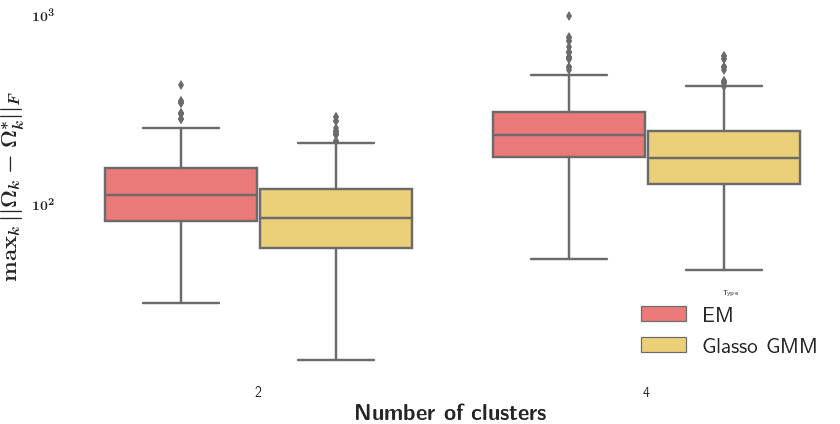
\includegraphics[width=0.8\textwidth]{TeX_files/graph_lasso_2_100.png} 
                \caption{p=2, N=100}
                \label{fig:glasso_dim2_N100}
        \end{subfigure}       
        \begin{subfigure}[b]{\textwidth}
                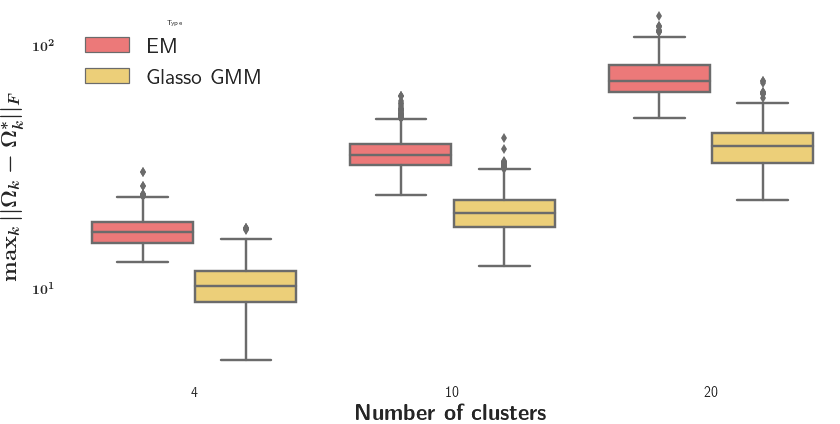
\includegraphics[width=0.8\textwidth]{TeX_files/graph_lasso_5_1000.png}
                \caption{p=5, N=1000}
                \label{fig:glasso_dim5_N1000}
        \end{subfigure}
        \caption{Estimation with glasso on GMM}\label{fig:glasso_res_simu} 
\end{figure}

\begin{figure}

        \begin{subfigure}[b]{\textwidth}
                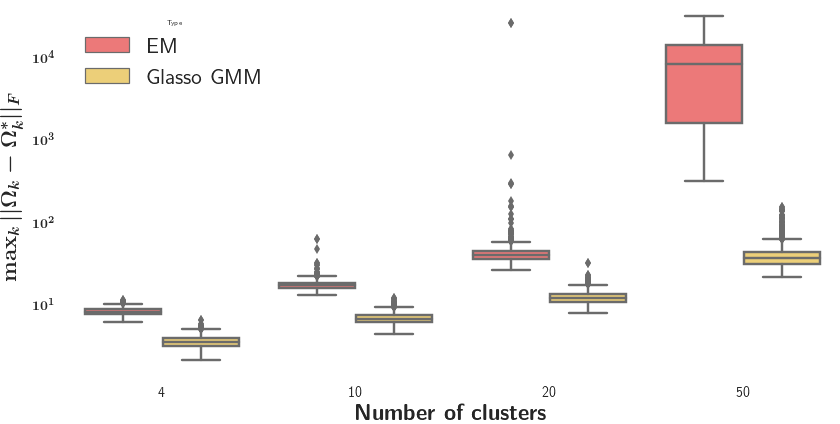
\includegraphics[width=0.8\textwidth]{TeX_files/graph_lasso_10_1000.png} 
                \caption{p=10, N=1000}
                \label{fig:glasso_dim10_N1000}
        \end{subfigure}       
        \begin{subfigure}[b]{\textwidth}
                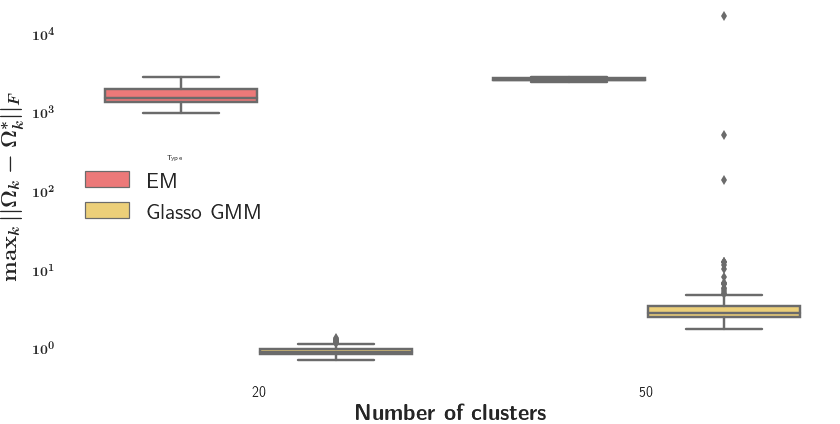
\includegraphics[width=0.8\textwidth]{TeX_files/graph_lasso_50_1000.png}
                \caption{p=50, N=1000}
                \label{fig:glasso_dim50_N1000}
        \end{subfigure}
        \caption{Estimation with glasso on GMM}\label{fig:glasso_res_simu2} 
\end{figure}

\begin{figure}

        \begin{subfigure}[b]{\textwidth}
                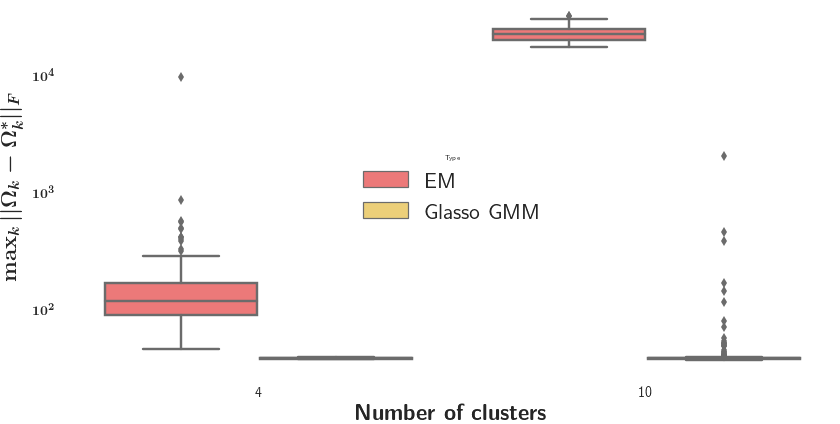
\includegraphics[width=0.8\textwidth]{TeX_files/graph_lasso_diag_upper10_100.png} 
                \caption{p=10, N=100, upper diag}
                \label{fig:glasso_dim10_N100_ud}
        \end{subfigure}       
        \begin{subfigure}[b]{\textwidth}
                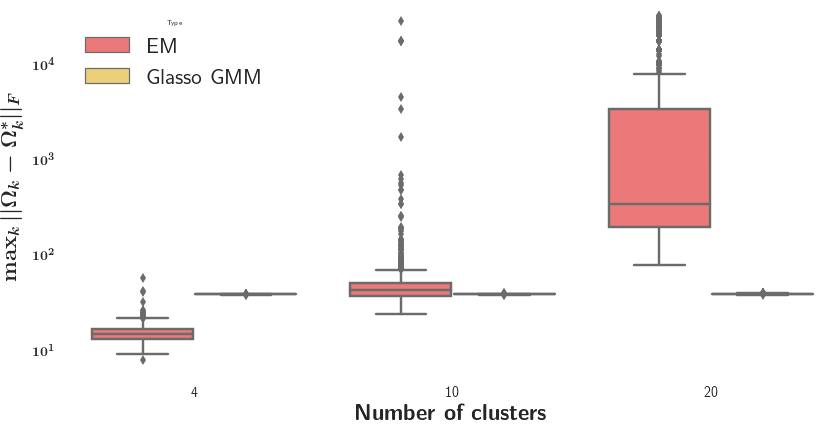
\includegraphics[width=0.8\textwidth]{TeX_files/graph_lasso_diag_upper10_500.png}
                \caption{p=10, N=500, upper diag}
                \label{fig:glasso_dim10_N500_ud}
        \end{subfigure}
        \caption{Estimation with glasso on GMM}\label{fig:glasso_res_simu2} 
\end{figure}
\begin{figure}

        \begin{subfigure}[b]{\textwidth}
                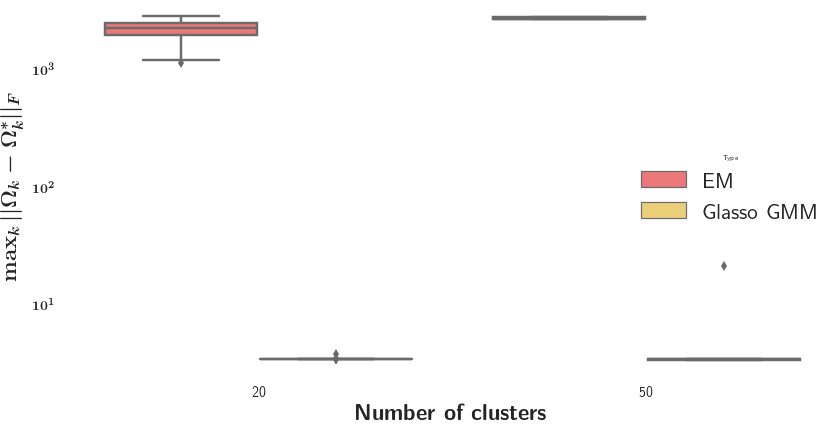
\includegraphics[width=0.8\textwidth]{TeX_files/graph_lasso_diag_upper50_1000.png} 
                \caption{p=50, N=1000, upper diag}
                \label{fig:glasso_dim50_N1000_ud}
        \end{subfigure}       
        \caption{Estimation with glasso on GMM}\label{fig:glasso_res_simu2} 
\end{figure}

\section{Estimating the number of clusters}
\label{estim_nb_clusters_sect}

In this section, we will focus on the problem of estimating the number of clusters, $K$, in a Gaussian mixture model. Most of popular clustering methods such as K-Means, Expectation-Maximization with Gaussian mixture model or spectral clustering need this parameter in input. Different methods are being used to perform a selection of the best model according to a criterion, unfortunately with a computational cost. As we saw in \Cref{sec:finding_clusters_nb}, we generally have to perform multiple clusterings with the parameter $K$ ranging from say 2 to $K_{max}$, where $K_{max}$ is a the maximum number of clusters we assume are present in the dataset, and select the best model according to a criterion. In this work, we seek to adapt the EM algorithm with an `adaptive' sparse estimation of the weight vector of the Gaussian components.

\subsection{First method: regularizing the posteriors}\label{sec:tau_pen_estim}
Our first approach was to penalize the matrix of posteriors $\bTau$ defined in \Cref{sec:EM_algo}. Given $N$ $p$-dimensional observations $\bx_1,\dots,\bx_N$, let us consider the EM algorithm with a number of clusters $K_{max}$ that we know is greater than the true number of clusters. The idea of this method is to add a regularization term on the estimation of the $N\times K_{max}$ matrix $\bTau$, the component $\tau_{i,j}$ of which, we recall, is defined as 
\begin{equation}
  \tau_{i,j} = p_{\btheta}(Z=j | \bX=\bx_i) = \frac{\pi_j\varphi_{\bmu_j,\bSigma_j}(\bx_i)}{\sum_{k=1}^{K_{max}}\pi_k\varphi_{\bmu_k,\bSigma_k}(\bx_i)}.
\end{equation}
The estimate number of clusters $\hat K$ will be the number of non-empty columns of $\bTau$. Let us consider the probability simplex in $\RR^{K_{max}}$, $\bPi\coloneqq \{\btau \in \RR^{K_{max}} : \sum_{k=1}^{K_{max}}\tau_k=1, \tau_k\geq 0 \quad \forall k \in [K_{max}] \}$ and the indicator function $\chi_{\bPi}(.)$ defined as
\begin{equation*}
    \chi_{\bPi}(\btau) =
    \begin{cases}
      0 & \text{if } \btau \in \bPi,\\
        +\infty & \text{elsewhere}.
    \end{cases}
\end{equation*}
We note $\bTau_{.,k}$ the $k^{th}$ column and $\bTau_{i,.}$ the $i^{th}$ line of $\bTau$. Using the cost function in \Cref{cost_gmm_em} and adding an $L_2$ penalization term of the columns of $\bTau$ with a parameter $\lambda > 0$, we have the following cost function for our problem:
\begin{align*}
F^{pen}(\btheta,\bTau)  =& -\sum_{k=1}^K \bigg(\sum_{i=1}^{n} \Big\{\tau_{i,k}\log\varphi_{\bmu_{k},\bOmega_{k}}(\bx_i)+\tau_{i,k}\log(\frac{\pi_k}{\tau_{i,k}})\Big\}\bigg)\\
&+ \lambda\sum_{k=1}^K \|\bTau_{.,k}\|_{2} + \sum_{i=1}^{n} \chi_{\bPi}(\bTau_{i,.}),
\end{align*}
 and the expectation step in EM consists on the following optimization problem:
\begin{equation}
\hat\bTau(\btheta)\in \argmin_{\bTau} F^{pen}(\btheta,\bTau).
\end{equation}
A nice property of this problem is that it is convex. Unfortunately, the regularization term prevents to derive an explicit solution. Furthermore, we cannot separate the objective function since we optimize along columns and lines of $\bTau$. The objective function $F^{pen}(\btheta,\bTau)$ rewritten $F^{pen}_{\btheta}(\bTau)$ can be split into two terms:
\begin{equation}
F^{pen}_{\btheta}(\bTau)={\large f}({\footnotesize\bTau})+ {\large g}({\footnotesize\bTau})
\end{equation}

with
\begin{align*}
f(\bTau) =& -\sum_{k=1}^K \bigg(\sum_{i=1}^{n} \Big\{\tau_{i,k}\log\varphi_{\bmu_{k},\bOmega_{k}}(\bx_i)+\tau_{i,k} \log(\pi_k/\tau_{i,k})\Big\} + \sum_{k=1}^K \|\bTau_{.,k}\|_{2},\\
g(\bTau) =& \sum_{i=1}^{n} \chi_A(\bTau_{i,.}).
\end{align*}
Note that $f$ is convex and differentiable on its domain, $g$ is also convex but not differentiable. We will tackle this problem by using a proximal method (see \citep{Parikh:2014:PA:2693612.2693613} for more details), the $(k+1)^{th}$ step is given by
\begin{align*}
  \bTau^{k+1} &= {\bf{prox}}_{g}(\bTau^k - \eta \nabla f(\bTau^k))\\
      &= \textnormal{P}_{\bPi}(\bTau^k - \eta \nabla f(\bTau^k))\\
      &=\argmin_{ \bTau : \forall i, \bTau_{i,.} \in \bPi}\big( \| \bTau - (\bTau^k - \eta \nabla f(\bTau^k) ) \|^2_2 \big),
\end{align*}
where $\textnormal{P}_{\bPi}$ is the projection function on $\bPi$. The gradient of f on $\bTau$ is given by
\begin{equation}
\bigg[\nabla_{\bTau}f(\bTau)\bigg]_{i,j} = 
1+\frac{\tau_{i,j}}{||\bTau_{.,j}||_2}-\log(\varphi_{\bmu_j,\bOmega_j}(\bx_i))-\log(\frac{\pi_j}{\tau_{i,j}})
\end{equation}
We use the algorithm FISTA \citep{Beck:2009:FIS:1658360.1658364} for this iteration procedure, we provide more details on this method in \Cref{mle_kl_estim_impl}. The implementation of this method is given in \Cref{algo:Pen_tau_EM_expect}, the whole EM-like method for the estimation of the parameters of the GMM is given in \Cref{algo:Pen_tau_EM}. 
\begin{figure}
\begin{center}
\mybox{
\begin{minipage}{0.85\linewidth}
\begin{algorithmic}%\SetAlgoLined\tt\SetLine
\small
\STATE {\bfseries Input:} Parameters $\btheta=(\bmu,\bSigma,\bpi)$
\STATE {\bfseries Output:} Estimate $\hat\bTau$
\STATE {\tt 1: Initialize $t_0=1$ and $\bxi^0$ with}
\begin{align*}
\xi_{i,k}^{0}  &= \frac{\pi_k^{0}\varphi_{\bmu_k^{0},\bOmega_k^{0}}(\bx_i)}{\sum_{k'\in[K]}\pi^{0}_{k'}\varphi_{\bmu^{0}_{k'},\bOmega^{0}_{k'}}(\bx_i)}
\end{align*}
\FOR{$k\geq 1,$ until convergence occurs, }
\STATE {(a) $\bTau^k =\argmin_{ \bTau : \forall i, \bTau_{i,.} \in \bPi}\big( \| \bTau - (\bxi^k - \lambda \nabla f(\bxi^k) ) \|^2_2 \big)$,}
\STATE {(b) $t_{k+1}= \frac{1+\sqrt{1+4t_k^2}}{2}$,}
\STATE {(c) $\bxi_{k+1} = \bTau^k + \bigg( \frac{t_k-1}{t_{k+1}}\bigg) \big( \bTau^k - \bTau^{k-1} \big)$.}
\ENDFOR
\end{algorithmic}
\end{minipage}}
   \caption{Expectation step, estimation of $\bTau$ with FISTA.}
   \label{algo:Pen_tau_EM_expect}
\end{center}
\end{figure}

\begin{figure}
\begin{center}
\mybox{
\begin{minipage}{0.85\linewidth}
\begin{algorithmic}%[1]\tt
%\SetLine%\SetAlgoLined
\small
\STATE {\bfseries Input:} Observations $\bx_1,\ldots,\bx_N\in\RR^p$ and the number of clusters $K$
\STATE {\bfseries Output:} Parameter estimate $\hat\btheta = \{\hat\bmu_k,\hat\bSigma_k,\pi_k\}_{k\in[K]}$
\STATE {\tt 1:} Initialize $t=0$, $\btheta=\btheta^0$.
\STATE {\tt 2:} {\bf Repeat}
\STATE \qquad {\tt 3:} Update the parameter $\bTau$ by using the procedure given in \Cref{algo:Pen_tau_EM_expect}.
\STATE \qquad{\tt 4:} Update the parameter $\btheta$:
\begin{align*}
\pi_k^{t+1}     &= \frac1N\sum_{i=1}^N \tau_{i,k}^t,\qquad
\bmu_k^{t+1}    = \frac1{N\pi_k^{t+1}}\sum_{i=1}^N \tau_{i,k}^t\bx_i,\\
\bSigma_k^{t+1} &= \frac1{N\pi_k^{t+1}}\sum_{i=1}^N \tau_{i,k}^t(\bx_i-\bmu_k^{t+1})(\bx_i-\bmu_k^{t+1})^\top.
\end{align*}
\STATE \qquad {\tt 5:} increment $t$: $t=t+1$.
\STATE {\tt 6:} {\bf Until} stopping rule.
\STATE {\tt 7:} {\bf Return} $\btheta^{t}$.
\end{algorithmic}
\end{minipage}}
   \caption{EM algorithm with penalization on the columns of $\bTau$.}
   \label{algo:Pen_tau_EM}
\end{center}
\end{figure}
A major drawback of this method is the computational cost in \Cref{algo:Pen_tau_EM_expect} of minimizing over the set of $N\times K_{max}$ matrices and we didn't manage to get interesting results for this algorithm.\todos{tentative de sortir des graphs en cours}

\subsection{Second method: penalizing the weights vector}
\label{sparse_weight_vect_estim}
The second approach that we took in order to have an estimate of the number of clusters, i.e. select an appropriate model, was to penalize the weights vector of the Gaussian mixture. The idea is similar to the previous method with an EM-like algorithm maximizing a penalized log-likelihood. Let $\lambda > 0$ be a parameter of penalization and consider the following negative penalized log-likelihood:
\begin{equation}
  \ell_N(\btheta)=
-\frac{1}{N}\sum_{i=1}^{N}\log\bigg\{{\sum_{j=1}^K\pi_k\varphi_{(\bmu_{j},\bSigma_{j})}(\bx_i)}\bigg\}+\lambda\sum_{j=1}^{K}\pi_j^{1/\gamma}\quad \gamma\geq1,
\end{equation}
such that:
\begin{equation}
  \forall j\in[K], \pi_j \geq 0 \quad \text{and} \quad \sum_{j}^{K}\pi_j=1.
\end{equation}
One may wonder why choosing such penalization ? The aim is to promote the merging of similar clusters. For instance, let us consider 2 similar clusters (similar means and covariance matrices) with a weight vector $\bpi=(1/2, 1/2)$ and the merged cluster with weight $\bpi'=(1)$. It is obvious that the log-likelihoods are the same. By choosing the $L_1$ norm, the weight vector $\pi_1+\pi_2$ leads to a penalty equal to 1 which is the same that taking the merged cluster with a weight and penalty equal to 1. However, by taking the penalty $\pi_1^{\nicefrac{1}{2}}+\pi_2^{\nicefrac{1}{2}}$ we have a penalty for the two clusters equal to $2/\sqrt{2}\sim 1.4$. Hence, the method will promote the solution with one cluster. Let us consider the $K$-dimensional probability simplex $\BB^+_K=\{\bpi\in \RR^K: \forall j\in[K], \pi_j \geq 0,\,  \sum_{j}\pi_j=1\}$. Our method is similar to EM in the expectation step and in the maximization step for estimating $\bmu_k$ and $\bSigma_k$, it differs on the estimation of the weights vector $\bpi$ by solving the following minimization problem:
\begin{equation}
  \hat\bpi= \argmin_{\bpi\in\BB^+_K}\bigg\{
-\frac{1}{N}\sum_{i=1}^{N}\log\Big({\sum_{j=1}^K\pi_k\varphi_{(\bmu_{j},\bSigma_{j})}(\bx_i)}\Big)+\lambda\sum_{j=1}^{K}\pi_j^{1/\gamma}\bigg\} \quad \gamma\geq1.
\end{equation}
Unfortunately, $\sum_{j}\pi_j^{1/\gamma}$ is not convex, we solve this problem by making a change of variable, let us note $\alpha_j = \pi_j^{1/\gamma}$ and consider the problem:
\begin{equation}
\hat\balpha\in\argmin_{\balpha\in \RR^{K}}\bigg\{
-\frac{1}{N}\sum_{i=1}^{N}\log\Big\{{\sum_{j=1}^K\alpha^\gamma_j\varphi_{(\bmu_{j},\bSigma_{j})}(\bx_i)}\Big\}+\lambda\sum_{j=1}^{K}\alpha_j \color{black} \bigg\}\quad \gamma\geq1,  
\end{equation}
with  $\forall j \in[K]\, \alpha_j^\gamma \geq0\ \text{and}\ \sum_{j}\alpha^\gamma_{K}=1$. This is a convex problem and we can recover an estimate $\hat\bpi=(\hat\alpha_1^{\gamma},\dots,\hat\alpha_K^{\gamma})$. The first term of this objective function is convex and differentiable with respect to $\balpha$, we note it $f_\btheta(\balpha)$. However, the second term, is convex but not differentiable w.r.t. $\balpha$. As we saw in the previous section, we can use an iterative proximal method to solve this problem. Let us consider $\gamma\geq 0$ and define $A_{\gamma}=\{\balpha\in\RR^K: \forall j \in[K]\, \alpha_j^\gamma \geq0\ \text{and}\ \sum_{j}\alpha^\gamma_{K}=1 \}$. If we consider {\large$\chi_{A_{\gamma}}$}, the indicator function of $A_{\gamma}$ ($0$ in $A_{\gamma}$, $\infty$ elsewhere), the minimization problem can be rewritten as
\begin{equation}
  \hat\balpha\in\argmin_{\balpha\in\RR^{K}}\{ f_\btheta(\balpha) + \chi_{A_{\gamma}}  \},
\end{equation}
and the $(t+1)^{th}$ step of the iterative proximal procedure is:
\begin{align}
\hat\balpha^{t+1}
&={\text{prox}}_{\chi_{A_{\gamma}}}( \balpha^t - h \nabla f_{\btheta}(\balpha^t)  )\\
&=\argmin_{x\in\RR^{K}}\Big\{ \chi_{A_{\gamma}}(x) + \frac{1}{2}\|x-(\balpha^t - h \nabla f_{\btheta}(\balpha^t)) \|^2 \Big\}\\
&=\textnormal{P}_{A_{\gamma}}(\balpha^t - h \nabla f_{\btheta}(\balpha^t) ),
\end{align}
with $h>0$ a gradient step, and for $j\in[K]$, the gradient of $f_{\btheta}$ w.r.t $\balpha$ is
\begin{equation}
  \Big[\nabla f_{\btheta}(\balpha)\Big]_{j} = -\frac{1}{N}\sum_{i=1}^N\frac{\gamma\alpha_j^{\gamma-1}\varphi_{\bmu_j,\bSigma_j}(\bx_i)}{\sum_{k=1}^K\alpha_k^{\gamma}\varphi_{\bmu_k,\bSigma_k}(\bx_i)}+\lambda.
\end{equation}
The FISTA procedure for estimating $\hat\balpha$ is given in \Cref{algo:alpha_fista_proc}. Note that we relaxed the constraints by estimating the $K-1$ components of $\balpha$ since $\alpha_K=1-\sum_{k=1}^{K-1}\alpha_k$. The set $A_{\gamma}$ is redefined accordingly: $A=\{\balpha\in\RR^{K}: \sum_{k=1}^{K-1}\alpha_k\leq1,\, \alpha_K=1-\sum_{k=1}^{K-1}\alpha_k\}$. The final EM-like iteration procedure for estimating the parameters of a Gaussian mixture with penalization of the weights vector is given in \Cref{algo:EM_alpha_pen}.
\begin{figure}[H]
\begin{center}
\mybox{
\begin{minipage}{0.85\linewidth}
\begin{algorithmic}%\SetAlgoLined\tt\SetLine
\small
\STATE {\bfseries Input:} Parameter $\btheta=\{(\bmu_k,\bSigma_k,\bpi)_{k\in[K]}\}$.
\STATE {\bfseries Output:} Parameter estimate $\hat\balpha = \big(\balpha_1,...,\balpha_{K-1},1-\sum_{j=1}^{K-1}\balpha_j).$
\STATE {\tt 1:} Initialize $t_0=1$ and $\xi^0=(\bpi_1^{1/\gamma},...,\bpi_{K-1}^{1/\gamma})$.
\FOR{$k\geq1$, until convergence occurs, }
\STATE {(a) $\balpha^k =\textnormal{P}_A(\xi^k - h \nabla f_{\btheta}(\xi^k))$,}
\STATE {(b) $t_{k+1} = \frac{1+\sqrt{1+4t_{k+1}^2}}{2}$}
\STATE {(c) $\bxi^{k+1} = \balpha^t + \bigg( \frac{t_k-1}{t_{k+1}}\bigg) \big( \balpha^k - \balpha^{k-1} \big)$}
\ENDFOR
\end{algorithmic}
\end{minipage}}
   \caption{Estimation of $\balpha$ via the FISTA method. }
   \label{algo:alpha_fista_proc}
\end{center}
\end{figure}
\begin{figure}[H]
\begin{center}
\mybox{
\begin{minipage}{0.85\linewidth}
\begin{algorithmic}%\SetAlgoLined\tt\SetLine
\small
\STATE {\bfseries Input:} Observations $\bx_1,\ldots,\bx_N\in\RR^p$ and a number of clusters $K_{max}$.
\STATE {\bfseries Output:} parameter estimate $\hat\btheta = \{\hat\bmu_k,\hat\bSigma_k,\hat\pi_k\}_{k\in[K]}$
\STATE {\tt 1:} Initialize $t=0$, $\btheta=\btheta^0$.
\FOR{$t=1,\dots$, until convergence occurs,}
\STATE {\tt 2:} Update the parameter $\bTau$:
\begin{equation*}
\tau_{i,k}^{t}  = \frac{\pi_k^{t}\varphi_{\bmu_k^{t},\bSigma_k^{t}}(\bx_i)}{\sum_{k'\in[K]}\pi^{t}_{k'}\varphi_{\bmu^{t}_{k'},\bSigma^{t}_{k'}}(\bx_i)}.
\end{equation*}
\STATE {\tt 3:} Update the parameter $\hat\balpha^{t+1}$ with algorithm in \Cref{algo:alpha_fista_proc} and compute $\hat\bpi^{t+1}=((\alpha_1^{t+1})^{\gamma}),\dots,(\alpha_K^{t+1})^{\gamma})$.
\STATE {\tt 4:} Update parameters $(\bmu_k,\bSigma_k)$ for $k\in[K_{max}]$:
\begin{align*}
\bmu_k^{t+1}    &= \frac1{n\pi_k^{t+1}}\sum_{i=1}^n \tau_{i,k}^t\bx_i,\\
\bSigma_k^{t+1} &= \frac1{n\pi_k^{t+1}}\sum_{i=1}^n \tau_{i,k}^t(\bx_i-\bmu_k^{t+1})(\bx_i-\bmu_k^{t+1})^\top.
\end{align*}
\ENDFOR
\end{algorithmic}
\end{minipage}}
   \caption{Algorithm for estimating sparse weights vector on GMM.}
   \label{algo:EM_alpha_pen}
\end{center}
\end{figure}
We generated different mixtures with $K$ varying from 2 to 30 components in dimension 5 and draw $N=1000$ observations. We compared our algorithm with EM and the BIC selection method with $K_{max}=2*K$. The resulting weight vectors are compared with the true weight $\bpi^*$ in $L_1$ norm. The plot of our simulations are given in \Cref{fig:results_alpha_pen}. In the horizontal axis, the number of real clusters in the mixture and in the vertical axis the error  $\|\hat\bpi-\bpi^*\|_1$. We ran 50 simulations, the first and third quartiles are shown as long as the median on each regions. As we can see, our algorithm shows promising results. With a small number of clusters, the estimation error $\|\hat\bpi-\bpi^*\|_1$ of our algorithm (green) is greater than with EM-BIC (red). However, when the number of clusters $K$ increases the estimation error of our algorithm decreases whereas the estimation error of EM-BIC increases. Such phenomenon of decreasing error while the complexity increase is not logical, we are confident that a more careful choice of the penalization parameter $\lambda$ would improve the error in low regime showing a slightly increasing curve, still better than EM-BIC.
\begin{figure}
\center
  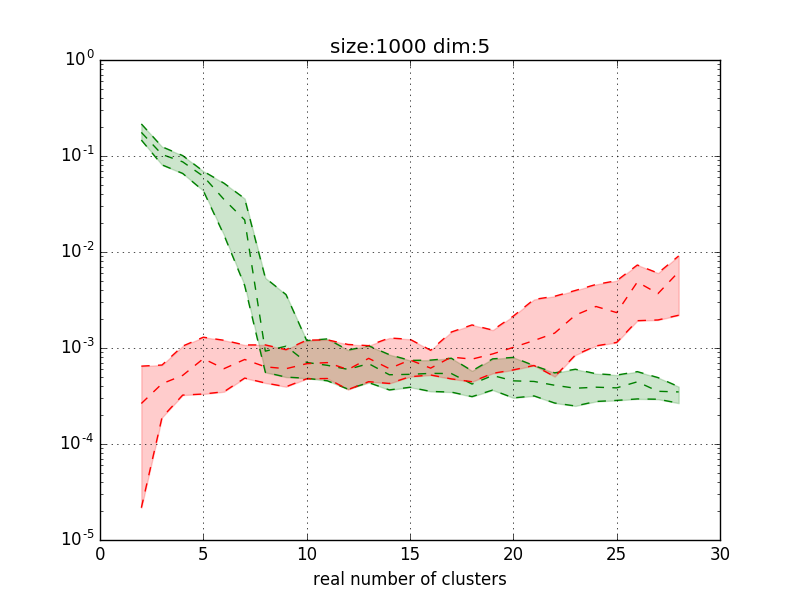
\includegraphics[scale=0.5]{./TeX_files/SparseWeightsVectorEstimation.png}
  \caption{Estimation error $\|\hat\bpi-\bpi^*\|_1$, for our algorithm (green) and EM-BIC (red). Vertical axis: error $\|\hat\bpi-\bpi^*\|_1$ in log scale, horizontal axis: real number of clusters. First and third quartiles are shown as long as the median.}
  \label{fig:results_alpha_pen}
\end{figure}
\todos{mentionner que cette approche est similaire avec les chapitres suivant sur le MLE}
